\documentclass[12pt, titlepage]{article}

\usepackage{booktabs}
\usepackage{tabularx}
\usepackage{graphicx}
\usepackage{hyperref}
\hypersetup{
    colorlinks,
    citecolor=black,
    filecolor=black,
    linkcolor=red,
    urlcolor=blue
}
\usepackage[round]{natbib}

\title{SE 3XA3: Software Requirements Specification\\DNA Says}
\author{Team 10, Team Name: DNA
		\\ Kareem Abdel Mesih (abdelk2)
		\\ John-Paul Dakran (dakranj)
		\\ Shady Nessim (nessimss)
}

\date{\today}

\begin{document}

\maketitle

\pagenumbering{roman}
\tableofcontents
\listoftables
\listoffigures

\begin{table}[bp]
\caption{\bf Revision History}
\begin{tabularx}{\textwidth}{p{3cm}p{2cm}X}
\toprule {\bf Date} & {\bf Version} & {\bf Notes}\\
\midrule
2016/10/10 & 1.0 & Completion of sub-section 1 \& 2\\
2016/10/10 & 2.0 & Completion of sub-section 4 \\
2016/10/11 & 3.0 & Completion of sub-section 3 \\
2016/12/02 & 4.0 & Revision 1 \\
\bottomrule
\end{tabularx}
\end{table}

\newpage

\pagenumbering{arabic}

\section{Project Drivers}

\subsection{The Purpose of the Project}
Video games have always been one of the top choices with regards to entertainment. They are also named as one of the great ways to overcome boredom. This project is a redevelopment of the famous digital game Simon Says, with a slight modification that makes DNA Says unique while keeping the integrity of the game consistent with the original version. This interactive game serves the purpose of allowing people of all ages, whether bored or simply having a break, to enjoy a fun and an interactive game. The main basis of Simon Says is to remember a given pattern, and iterate it back. In addition, this project will aid in the enhancement of ones visual and auditory memory.
\subsection{The Stakeholders}

\subsubsection{The Client}
This pogram is developped as the final project for McMaster University's Software Engineer 3XA3 - Software Project Management. Therefore, the client for this project is Dr. Spencer Smith, the  Professor of  that course.

\subsubsection{The Customers}
The customers for this project are the general public who will operate the game DNA Says. A typical customer will be any person ranging from five years of age and older, who can access and operate a computer. 

\subsubsection{Other Stakeholders}
\begin{itemize}
\item The Development Team - Kareem, John-Paul and Shady.
\item Previous and future developers as they possess the power to modify and publish this program as they desire.
\end{itemize}

\subsection{Mandated Constraints}

\subsubsection{Solution Constraints}
Description: This game is OS independant. It is compatible with Windows, Mac OS X, and Linux operating systems.\\
\\
Rationale: The client will be using any of the operating systems listed above.\\
\\
Fit Criterion: During the user testing phase, all of the operating systems mentioned above were tested.

\subsubsection{Partner or Collaborative Applications}
This project is a redevelopment of the digital game Simon Says in which its Python open source code is available online. The new game DNA Says supports the current game's user platform.

\subsubsection{Budget Constraints}
The operating budget of the project is \$0. All resources needed to develop this game are currently owned by the developers.

\subsubsection{Scheduling Constraints}
The project must be fully completed by December 7, 2016. This includes the implementation, testing and documentation.

\subsubsection{Enterprise Constraints}
This game is free and accessible to all users who have exposure to a computer. 

\subsection{Naming Conventions and Terminology}
.
\begin{table}[h!]
	\centering
	\caption{List of Terminology}
	\label{tab:table3}
	\begin{tabular}{ll}
		\hline
		Term & Definiton\\
		\hline
		OS & Short for operating systems.\\
		Windows & Microsoft's operating system.\\
		Mac OS X & Apple's operating system.\\
		Linux & A Unix operating system.\\
		Python & A programming language.\\
		IDLE & Integrated development environment\\
		LaTeX & A document preparation system. \\
		Mode & Different subsections of the game.\\
		GUI & Graphical user interface.\\
		Gantt Chart & Chart outlining the timeline of the project.\\
		\hline
	\end{tabular}
\end{table}

\subsection{Relevant Facts and Assumptions}
\subsubsection{Relevant Facts}

Python is used to develop this project. It runs in its basic IDLE Version 3.5. Framework is tested in an automated fashion to validate the different cases and outcomes of the game. Family and friends have tested the overall functionality and performance of the game, as well as its non-functional requirements. LaTeX is to generate required documents.\\
\\
The previous implementation of this game has approximately two hundred and fifty lines of code. That implementation only has one mode, however the version implemented has three different modes and a menu. Therefore the number of lines of code is greater than the original version's. The original implementation has no licenses that need to be acquired by the team or McMaster University.

\subsubsection{Assumptions}
It is assumed that the user has downloaded any version of Python along with its corresponding Pygame version.
\\
It is also assumed that the user has basic understanding of operating a computer. The user must be able to open an application and follow simple instructions to interact with the GUI.\\
\\
Finally, the user's computer must have enough processing speed and storage to effectively run and host the application.

\section{Functional Requirements}
\subsection{The Scope of the Work and the Product}

\subsubsection{The Context of the Work}
.
\begin {figure}[h]
	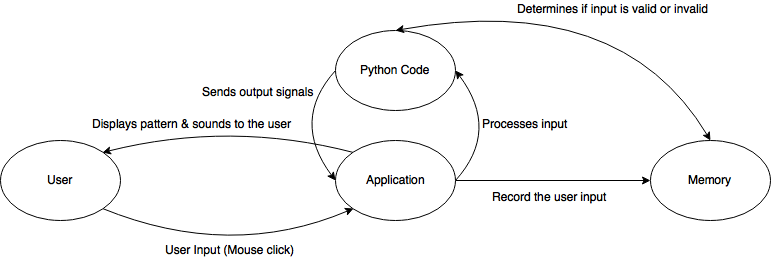
\includegraphics [width = \linewidth] {Context_Of_Work.png}
	\caption {Context of Work Diagram}
	\label {Figure: Context of Work}
\end {figure}

\newpage
\subsubsection{Work Partitioning}

\begin{table}[h]
	\centering
	\caption{List of Events}
	\label{tab:table2}
	\begin{tabular}{clll}
		\hline
		\# & Event & Input & Output\\
		\hline
		1. & DNA Says Creation & Developer code & Executable file\\
		2. & DNA Says Audio & None & Audio output device\\
		3. & DNA Says GUI & Developer code & Monitor\\
		4. & Open the file & User input & New window\\
		5. & Select a mode & User input & Buttons appear\\
		6. & Click a correct disk & User input & Light \& sound\\
		7. & Click an incorrect disk & User input & Light \& sound\\
		8. & Repeat pattern successfully & User input & Addition to the pattern\\
		9. & Exit to main menu & User input & Main menu appears\\
		10. & Exit game & User input & Window termination\\
		\hline
	\end{tabular}
\end{table}


\subsubsection{Individual Product Use Cases}

\begin{itemize}

\item Use Case \#1
\begin{itemize}
\item Name: Open the executable file.
\item Trigger: The user selects to open the file.
\item Precondition: The DNA Says icon must be available on the desktop.
\item Postcondition: The main menu will open.
\end{itemize}

\item Use Case \#2
\begin{itemize}
\item Name: Select a mode.
\item Trigger: The user selects to choose one of the three modes.
\item Precondition: The user must be in the main menu.
\item Postcondition: The user will be able to view the three buttons and begin the game.
\end{itemize}

\item Use Case \#3
\begin{itemize}
\item Name: Click a correct button.
\item Trigger: The user selects a button that was part of the pattern displayed in the correct playing order. 
\item Precondition: The user must be in a mode and the computer has displayed the pattern.
\item Postcondition: The button will light up and make a sound.
\end{itemize}

\item Use Case \#4
\begin{itemize}
\item Name: Click an incorrect button.
\item Trigger: The user selects a button that was not part of the pattern displayed.
\item Precondition: The user must be in a mode and the computer has displayed the pattern.
\item Postcondition: The game will make a specific sound indicating an incorrect move and the screen will flash.
\end{itemize}

\item Use Case \#5
\begin{itemize}
\item Name: Successfully repeat the pattern.
\item Trigger: The user selects the series of button that composed the pattern displayed in order.
\item Precondition: The user must be in a mode and the computer has displayed the pattern.
\item Postcondition: The next pattern will be displayed to the user.
\end{itemize}

\item Use Case \#6
\begin{itemize}
\item Name: Exit to the main menu.
\item Trigger: The user selects main menu icon.
\item Precondition: The user must be in a mode. 
\item Postcondition: The user will leave a mode and the main menu will open.
\end{itemize}

\item Use Case \#7
\begin{itemize}
\item Name: Exit game.
\item Trigger: The user selects the exit game icon
\item Precondition: The user must be in the main menu. 
\item Postcondition: The appllicaion will be terminated
\end{itemize}

\end{itemize}




\section{Functional Requirements}

\begin{itemize}

\item Requirement \#1
\begin{itemize}
\item Description: The user will be able to open the executable file.
\item Rationale: The user must be able to open the program.
\item Fit Criterion: A new window will open on the user's computer screen.
\end{itemize}

\item Requirement \#2
\begin{itemize}
\item Description: The  interface will open in a new window.
\item Rationale: The program will be operated in a separate window. 
\item Fit Criterion: A new window will appear on the user's computer screen
\end{itemize}

\item Requirement \#3
\begin{itemize}
\item Description: The game will have three separate modes - Kareem Says, JP Says and Shady Says.
\item Rationale: The game is designed to have three distinct modes.
\item Fit Criterion: The three different modes will be displayed on the main menu of the game. 
\end{itemize}

\item Requirement \#4
\begin{itemize}
\item Description: The user will be able to select one of the three modes to play.
\item Rationale: The user must be able to play one mode at a time. 
\item Fit Criterion: The user will be able to select one of the three modes displayed in the main menu of the game.
\end{itemize}

\item Requirement \#5
\begin{itemize}
\item Description: The main menu will display the three different modes. 
\item Rationale: The user must be able to view which mode they wish to select.
\item Fit Criterion: Three distinct icons will be displayed in the main menu.
\end{itemize}

\item Requirement \#6
\begin{itemize}
\item Description: If Kareem Says is selected, then a piano will be displayed on the screen, otherwise nine squared buttons will show up for JP Says, and four for Shady Says.
\item Rationale: The game is designed to have different interfaces for each mode.
\item Fit Criterion: When a user selects a mode - accordingly, a piano will show up, nine buttons or four buttons. 
\end{itemize}

\item Requirement \#7
\begin{itemize}
\item Description: Each button will light up and produce a different sound when clicked.
\item Rationale: This gives the user the ability to detect the pattern that will be displayed.
\item Fit Criterion: When the user clicks a button, the button will light up and produce a sound.
\end{itemize}

\item Requirement \#8
\begin{itemize}
\item Description: The user will be able to exit the game at any time and go back to the main menu. 
\item Rationale: The user must have a means of exiting an ongoing game and return to the main menu.
\item Fit Criterion: When the user clicks the main menu button, they will find their screen in the main menu window.
\end{itemize}

\item Requirement \#9
\begin{itemize}
\item Description: Every time a user passes a level, the score goes up by one point.
\item Rationale: A record of a user's score must be kept. 
\item Fit Criterion: At level N, the score = N.
\end{itemize}

\item Requirement \#10
\begin{itemize}
\item Description: Every time a user fails a level, the score is reset to zeo.
\item Rationale: When a user fails a level, the game must restart from level one.
\item Fit Criterion: Whenever the user makes a mistake, the score text will reset to zero.
\end{itemize}

\item Requirement \#11
\begin{itemize}
\item Description: There will be a score icon in the top right corner.
\item Rationale: The user must be able to view their score.
\item Fit Criterion: When the user selects a mode, the score icon will be set to zero.
\end{itemize}

\item Requirement \#12
\begin{itemize}
\item Description: At level N, a random pattern of N disks will light up and be displayed to the user.
\item Rationale: The pattern's length will increase as the levels progress.
\item Fit Criterion: During level one, one random button will light up and sound.
\end{itemize}

\item Requirement \#13
\begin{itemize}
\item Description: The user cannot click the button while the pattern is being displayed. 
\item Rationale: The pattern must be displayed to the user in full effect.
\item Fit Criterion: The program will not record clicks the user inputs during this time.
\end{itemize}

\item Requirement \#14
\begin{itemize}
\item Description: The user will be able to click the buttons once the pattern has been displayed. 
\item Rationale: The user must repeat the pattern correctly to pass the level.
\item Fit Criterion: The program will monitor the user's input clicks to determine if the entry is correct or not.
\end{itemize}

\item Requirement \#15
\begin{itemize}
\item Description: A level is passed if the user repeats the pattern correctly.
\item Rationale: The user will be able to progress through the game. 
\item Fit Criterion: The score will be increased by 1 when the user is successful.
\end{itemize}

\item Requirement \#16
\begin{itemize}
\item Description: If the user fails, the game will restart - I.e. N = 1.
\item Rationale: The user must restart from the beginning of the game when a mistake is made.
\item Fit Criterion: Whenever a mistake is made, the user will be directed to level one.
\end{itemize}

\end{itemize}


\section{Non-functional Requirements}
\subsection{Look and Feel Requirements}
\subsubsection{Appearance Requirements}

\begin{itemize}

\item Requirement \#1 
\begin{itemize}
\item Description: The product shall have an appealing colorful appearance.
\item Rationale: The display should always be engaging so as to keep user interested in game. The product must be aesthetically pleasing and easy to use to benefit the end-users
\item Originator: Shady Nessim 
\item Fit Criterion: Stakeholder satisfaction regarding the appearance, user attraction to game. 
\item Priority: High 
\item History: Created October 5, 2016 \\
\end{itemize}

\item Requirement \#2 
\begin{itemize} 
\item Description: The buttons must be well designed and colored.
\item Rationale: The game revolves around pressing buttons in a pattern. It is the main entity of the game and must thus be aesthetically pleasing to attract user interest
\item Originator: Shady Nessim 
\item Fit Criterion: User reaches high levels as a result of uniqueness and beauty of buttons. 
\item Priority: High 
\item History: Created October 5, 2016 \\
\end{itemize}

\item Requirement \#3 
\begin{itemize} 
\item Description: The product shall have attractive sound patterns. The associated sounds with buttons must be well constructed and notes must follow harmonically.
\item Rationale: The user follows a pattern based on colors and sounds, the sounds must thus be well designed to be easy to follow. When user hears an attractive pattern, naturally they are inclined to repeat it.
\item Originator: Shady Nessim 
\item Fit Criterion: User shall be invested in game and spend a lot of time playing the game. 
\item Priority: High 
\item History: Created October 5, 2016 \\
\end{itemize}

\end{itemize}

\subsubsection{Style Requirements}
\begin{itemize} 

\item Requirement \#4 
\begin{itemize} 
\item Description: The product shall have enough buttons to keep game engaging but not too many as to make the screen feel cluttered. DNA Says will appear to be a bright upbeat game. 
\item Rationale: The game must induce a style and feel to the user that will be a driving factor to use the game if the user likes the style of the game
\item Originator: Shady Nessim 
\item Fit Criterion: Stakeholder satisfaction regarding the style, user attraction to game. 
\item Priority: Medium 
\item History: Created October 5, 2016
\end{itemize}

\end{itemize}

\subsection{Usability and Humanity Requirements}
\subsubsection{Ease of Use Requirements}
\begin{itemize}

\item Requirement \#5
\begin{itemize}  
\item Description: The product shall be easy to use for people of all ages, including children. 
\item Rationale: The game involves no reading or writing, it does not involve intelligence either. The game involves short term memory. As such it should be easy to use for all people to improve their short term memory.
\item Originator: Shady Nessim 
\item Fit Criterion: User figures out how to play the game within the first couple of minutes of use. 
\item Priority: High 
\item History: Created October 5, 2016
\end{itemize}

\item Requirement \#6
\begin{itemize}  
\item Description: The product shall be easy to install for all users. 
\item Rationale: This product is simply a game so the user will probably not go through the trouble of downloading and installing the game if it is not an easy process.
\item Originator: Shady Nessim 
\item Fit Criterion: User easily downloads and installs the game in a timely manner. 
\item Priority: High 
\item History: Created October 5, 2016
\end{itemize}

\end{itemize}

\subsubsection{Personalization and Internationalization Requirements}
\begin{itemize} 

\item Requirement \#7
\begin{itemize} 
\item Description: The product shall operate with the English language. 
\item Rationale: The application is intended for use by English and non-English speakers, however with minimal required text use, this game can easily be figured out and used by non-English speakers
\item Originator: Shady Nessim 
\item Fit Criterion: User easily understands objective of game and how to play. 
\item Priority: Medium 
\item History: Created October 5, 2016
\end{itemize}

\end{itemize}

\subsubsection{Learning Requirements}
\begin{itemize} 

\item Requirement \#8 
\begin{itemize} 
\item Description: The application shall not require a tutorial and shall be clear and simple enough in early levels to communicate to the user how the game is played.
\item Rationale: The application is intended for use by people of all ages. Must thus be easy to understand.
\item Originator: Shady Nessim 
\item Fit Criterion: User easily understands objective of game and how to play. 
\item Priority: Medium 
\item History: Created October 5, 2016
\end{itemize}

\end{itemize}

\subsubsection{Understandability and Politeness Requirements}
\begin{itemize}

\item Requirement \#9
\begin{itemize}  
\item Description: The application shall not produce ugly sound patterns or offensive visual patterns to respect all users.
\item Rationale: The application is intended for entertainment and as a cure for boredom, if user feels uncomfortable or offended they will not use the game.
\item Originator: Shady Nessim 
\item Fit Criterion: User feels good about game and patterns are appealing and attractive. 
\item Priority: Medium 
\item History: Created October 5, 2016
\end{itemize}

\item Requirement \#10
\begin{itemize} 
\item Description: The product shall produce a friendly indication when user loses or wins a level.
\item Rationale: The application is intended for entertainment and as a cure for boredom, if user feels uncomfortable or offended they will not use the game.
\item Originator: Shady Nessim 
\item Fit Criterion: User feels good about level progression and is encouraged to play again. 
\item Priority: Medium 
\item History: Created October 5, 2016
\end{itemize}

\end{itemize}

\subsubsection{Accessibility Requirements}
\begin{itemize} 

\item Requirement \#11
\begin{itemize} 
\item Description: The product shall produce patterns both visually and auditory so as to accommodate for users with visual or auditory problems that they can use an alternative pattern means.
\item Rationale: The application is intended all users, should be easy to use for someone by just following visual patterns or just following auditory patterns.
\item Originator: Shady Nessim 
\item Fit Criterion: User with auditory or visual problems feel comfortable playing the game. 
\item Priority: Medium 
\item History: Created October 5, 2016
\end{itemize}

\end{itemize}

\subsection{Performance Requirements}
\subsubsection{Speed and Latency Requirements}
\begin{itemize}

\item Requirement \#12 
\begin{itemize} 
\item Description: The application should be able to recognize whether the user has entered the right pattern as soon as they finish pressing the last button.
\item Rationale: The user should not have to wait for the application to calculate whether their input was correct or not.
\item Originator: Shady Nessim 
\item Fit Criterion: Application should respond immediately to user input and the upcoming pattern should start soon after user input ends.
\item Priority: High 
\item History: Created October 5, 2016
\end{itemize}

\end{itemize}

\subsubsection{Safety Critical Requirements}
There are none applicable to this project.

\subsubsection{Precision of Accuracy Requirements}
\begin{itemize}

\item Requirement \#13 
\begin{itemize} 
\item Description: The application must be specific to each button press. Button press confusion or mistake must not be tolerated.
\item Rationale: The purpose of the game is to produce exact same pattern shown by application. If program does not detect a mistake even if it is just one wrong button, then that defeats the fairness and purpose of the game.
\item Originator: Shady Nessim 
\item Fit Criterion: Application should perceive and evaluate user pattern input impeccably.
\item Priority: High 
\item History: Created October 5, 2016
\end{itemize}

\end{itemize}

\subsubsection{Reliability and Availability Requirements}
\begin{itemize} 

\item Requirement \#14 
\begin{itemize} 
\item Description: The application must be available at all times.
\item Rationale: The purpose of the game is to defeat boredom which may come at any time and thus the game must be available at all times.
\item Originator: Shady Nessim 
\item Fit Criterion: User should be able to play the game whenever they are bored.
\item Priority: High 
\item History: Created October 5, 2016
\end{itemize}

\end{itemize}

\subsubsection{Capacity Requirements}
\begin{itemize}

\item Requirement \#15 
\begin{itemize} 
\item Description: The application must be able to produce and receive patterns as long as 25 buttons.
\item Rationale: In order to make the game challenging enough, patterns including but not limited to 25 in length should be produced and received by program.
\item Originator: Shady Nessim 
\item Fit Criterion: User should be able to reach level 25 in each mode.
\item Priority: Medium 
\item History: Created October 5, 2016
\end{itemize}

\end{itemize}

\subsubsection{Scalability Requirements}
There are none applicable to the project.

\subsubsection{Longevity Requirements}
There are none applicable to the project.

\subsection{Operational and Environmental Requirements}
\subsubsection{Expected Physical Environment}
\begin{itemize}

\item Requirement \#16
\begin{itemize} 
\item Description: The product should be able to be used on laptops and desktops. 
\item Rationale: The clients will use the product from these devices.
\item Originator: Shady Nessim 
\item Fit Criterion: User should be able to run the game on any laptop or desktop.
\item Priority: High 
\item History: Created October 8, 2016
\end{itemize}

\end{itemize}

\subsubsection{Release Requirements}
\begin{itemize} 

\item Requirement \#17
\begin{itemize} 
\item Description: The product will be revised yearly and updated according to changing demands and needs of the client. The product will undergo maintenance upon realization of any errors in gameplay behavior.
\item Rationale: The game has to stay updated and problems have to be handled in order to maintain user interest and usage.
\item Originator: Shady Nessim 
\item Fit Criterion: App should be updated at least annually.
\item Priority: Medium 
\item History: Created October 8, 2016
\end{itemize}

\end{itemize}

\subsection{Maintainability and Support Requirements}
\subsubsection{Maintenance Requirement}
\begin{itemize}

\item Requirement \#18
\begin{itemize} 
\item Description: The source code for the application shall be visible to the public. 
\item Rationale: This enhances the ability to monitor and maintain the system. 
\item Originator: Shady Nessim
\item Fit Criterion: Source code is available in a public repository. 
\item Priority: Low 
\item History: Created October 10, 2016
\end{itemize}

\end{itemize}

\subsubsection{Supportability Requirements}
None applicable for this project.

\subsubsection{Adaptability Requirements}
\begin{itemize} 

\item Requirement \#19
\begin{itemize} 
\item Description: The product shall run on Windows, Linux and Mac OS X environments.
\item Rationale: The users may be using any of these operating systems.
\item Originator: Shady Nessim 
\item Fit Criterion: The product works on listed platforms in the test groups.
\item Priority: Medium 
\item History: Created October 10, 2016
\end{itemize}

\end{itemize}

\subsection{Security Requirements}
\subsubsection{Privacy Requirements}
\begin{itemize} 

\item Requirement \#20
\begin{itemize} 
\item Description: The application shall not store, transmit, or upload any user data.
\item Rationale: This is required in order to protect the privacy of users.
\item Originator: Shady Nessim
\item Fit Criterion: No functionality to perform these tasks is implemented in the application. 
\item Priority: Low 
\item History: Created October 10, 2016
\end{itemize}

\end{itemize}

\subsection{Cultural Requirements}
\begin{itemize}

\item Requirement \#21
\begin{itemize} 
\item Description: The application shall not contain any imagery or text that can be reasonably foreseen as potentially offensive to users of all cultures, backgrounds and ethnicities. 
\item Rationale: User satisfaction will be greatly reduced if they notice any offensive patterns in the game. 
\item Originator: Shady Nessim
\item Fit Criterion: Application does not contain offensive patterns or references. 
\item Priority: Medium 
\item History: Created October 10, 2016
\end{itemize}

\end{itemize}

\subsection{Legal Requirements}
There are none applicable to this project.




\section{Project Issues}

\subsection{Open Issues}
There has been no open issues in the duration of this project. The undocumented code has been carefully anlyzed and each line has been assessed and a solid understanding of the program has been gained.

\subsection{Off-the-Shelf Solutions}
In general, there are many games that share the similar nature and purpose. However, with respect to Simon Says, there is the original oral game in which one designated person speaks out an action for the others to do, having them only do the action if they say ?Simon says? before it. As for digital versions, there exists multiple ones online.

\subsection{New Problems}
The only problem that could arise from this project is addiction. As there could be individuals that instead of enjoying this game during their free time or as a short break from their schedule, they would consume their other priorities? time to play. This game could potentially be the reason behind a missed deadline, or anything in that manner.

\subsection{Tasks}
All tasks that need to be accomplished are covered within this group's Gantt Chart, including their start and end dates found here:

\begin{itemize}
\item \href{run:GanttChart.gan} {Gantt Chart}\\
\end{itemize}

\subsection{Migration to the New Product}
There will not be issues transferring from another version of this game to this current version. Only the user's preferences matter for this, and that will be discussed as a risk in the section below.

\subsection{Risks}
The initial risk has been that the user's preferences might conflict with the team's preferences that the game was built upon. That risk has been taken into consideration and to counter it, the team has developed a user survey. That survey was taken by various users that played the game and their opinions were analyzed and the game has been updated accordingly.

\subsection{Costs}
There are no monetary costs included in this project.

\subsection{User Documentation and Training}
Instructions are always available at the bottom left corner of the screen. The game is very simple and does not require more than one line of explanation per mode.

\subsection{Waiting Room}
At this point, the team is improving all documentation for the next round of marking.

\subsection{Ideas for Solutions}
To make sure that most of the users will enjoy this game, a survey was conducted to collect different thoughts and preferences as to what the users would like to see in this game, what they are looking forward to, and what they expect. That survey included the desired colors, sounds, interface and functionality. The current implementation of this project is modified to suit those preferences.

\bibliographystyle{plainnat}
\bibliography{SRS}
\newpage
\section{Appendix}
This section contains no related information for this document.
\subsection{Symbolic Parameters}
N represents any integer and does not have an upper bound. It is used throughout the document to represent level numbers, the number of elements in a given pattern and the score.
\end{document}